% A0 conference poster for AnomalyAgent
% Build once: ./render_poster.sh --once | Live rebuild: ./render_poster.sh
\documentclass[final]{beamer}

\usepackage[orientation=portrait,size=a0,scale=0.92]{beamerposter}
\usetheme{gemini}
\usecolortheme{nott}
\usepackage{graphicx}
\usepackage{booktabs}
\usepackage{array}
\usepackage{multirow}
\usepackage{amsmath}
\usepackage{ragged2e}
\usepackage{anyfontsize}
\usepackage{xcolor}
\usepackage{colortbl}
\usepackage{hyperref}
\usepackage{tikz}

% ==================== Visual identity ====================
\definecolor{agentnavy}{HTML}{10263B}
\definecolor{agentcyan}{HTML}{00A6C8}
\definecolor{agentorange}{HTML}{F28C28}
\definecolor{agentlight}{HTML}{EEF8FA}
\definecolor{agentwarm}{HTML}{FFF4E8}

\setbeamercolor{headline}{fg=agentnavy,bg=white}
\setbeamercolor{headline rule}{bg=agentcyan}
\setbeamercolor{block title}{fg=white,bg=agentnavy}
\setbeamercolor{block separator}{bg=agentcyan}
\setbeamercolor{block alerted title}{fg=agentnavy,bg=agentwarm}
\setbeamercolor{block alerted separator}{bg=agentorange}
\setbeamercolor{block alerted body}{fg=black,bg=agentwarm}
\setbeamercolor{block example title}{fg=agentnavy,bg=agentlight}
\setbeamercolor{block example separator}{bg=agentcyan}
\setbeamercolor{block example body}{fg=black,bg=agentlight}
\setbeamercolor{item}{fg=agentcyan}

\setbeamerfont{headline title}{size=\fontsize{50}{57},series=\bfseries}
\setbeamerfont{headline author}{size=\fontsize{26}{31}}
\setbeamerfont{headline institute}{size=\fontsize{19}{23}}
\setbeamerfont{block title}{size=\fontsize{44}{50},series=\bfseries}
\setbeamerfont{block body}{size=\fontsize{36}{45}}
\setbeamerfont{block alerted body}{size=\fontsize{30}{37}}
\setbeamerfont{block example body}{size=\fontsize{30}{37}}
\setbeamerfont{caption}{size=\fontsize{17}{20}}
\setbeamerfont{footline}{size=\fontsize{26}{32}}

% White-on-navy section bands with a restrained offset shadow.
% The band uses the existing width: figure sizes and table scales are unchanged.
\setbeamertemplate{block begin}{%
  \par\noindent
  \begin{tikzpicture}
    \path[fill=agentnavy!35,rounded corners=0.18cm]
      (0,-0.16cm) rectangle (\linewidth,2.04cm);
    \path[fill=agentnavy,rounded corners=0.18cm]
      (0,0) rectangle (\linewidth,2.2cm);
    \path[fill=agentcyan] (0.3cm,0.4cm) rectangle (0.42cm,1.8cm);
    \node[anchor=west,text=white,inner sep=0pt]
      at (0.85cm,1.1cm) {\usebeamerfont{block title}\insertblocktitle};
  \end{tikzpicture}\par
  \vspace{0.7cm}
  \usebeamerfont{block body}
  \begin{beamercolorbox}{block body}
  \setlength{\parskip}{0.45cm}}
\setbeamertemplate{block end}{\end{beamercolorbox}\vspace{0.8cm}}
\newcommand{\lead}[1]{{\color{agentnavy}\bfseries #1}}

% ==================== Asymmetric 1+2 column grid ====================
\newlength{\sepwidth}
\newlength{\colwidth}
\newlength{\twocolwidth}
\newlength{\widewidth}
\setlength{\sepwidth}{0.0125\paperwidth}
\setlength{\colwidth}{0.3166667\paperwidth}
\setlength{\twocolwidth}{0.6458333\paperwidth}
\setlength{\widewidth}{0.975\paperwidth}
\newcommand{\separatorcolumn}{\begin{column}{\sepwidth}\end{column}}
\newcommand{\tightlist}{\setlength{\itemsep}{0.3em}\setlength{\parskip}{0pt}}

\pdfmapfile{+libertine.map}
% Split directly from the paper's localization table; values and bold retained.
\newcommand{\PixelLocalizationTable}{%
\begingroup
\fontencoding{T1}\fontfamily{LinuxLibertineT-TLF}\fontseries{m}\fontsize{9}{10.8}\selectfont
\setlength{\tabcolsep}{1.5pt}
\renewcommand{\arraystretch}{1}
\centering
\resizebox{\linewidth}{!}{%
\begin{tabular}{l | ccc | ccc | ccc | ccc}
\toprule
\multicolumn{13}{c}{\textbf{Pixel-Level Performance}} \\
\midrule
\multirow{2}{*}{\textbf{Category}} & \multicolumn{3}{c|}{AnoHybrid} & \multicolumn{3}{c|}{Gemini-img} & \multicolumn{3}{c|}{GPT-img} & \multicolumn{3}{c}{\textbf{AnomalyAgent}} \\
\cmidrule(lr){2-4}\cmidrule(lr){5-7}\cmidrule(lr){8-10}\cmidrule(lr){11-13}
 & AUC & AP & \textit{F}\textsubscript{1} & AUC & AP & \textit{F}\textsubscript{1} & AUC & AP & \textit{F}\textsubscript{1} & AUC & AP & \textit{F}\textsubscript{1} \\
\midrule
bottle & 98.3 & \textbf{77.2} & \textbf{72.5} & 96.1 & 74.5 & 68.1 & 86.0 & 52.7 & 51.5 & \textbf{97.2} & 73.5 & 69.7 \\
cable & 94.1 & 76.0 & \textbf{73.4} & 93.3 & 68.5 & 60.2 & 90.2 & 55.5 & 50.4 & \textbf{97.4} & \textbf{76.5} & 69.2 \\
capsule & \textbf{98.4} & \textbf{51.7} & \textbf{54.6} & 96.0 & 44.0 & 47.3 & 88.3 & 33.2 & 34.5 & 96.6 & 46.0 & 49.7 \\
carpet & 98.6 & 82.8 & 75.6 & 98.8 & 79.0 & 72.3 & 91.3 & 69.0 & 60.4 & \textbf{99.4} & \textbf{85.1} & \textbf{76.4} \\
grid & \textbf{98.8} & \textbf{58.6} & \textbf{59.2} & 97.4 & 27.5 & 38.6 & 89.0 & 22.1 & 32.7 & 97.8 & 40.3 & 44.9 \\
hazelnut & \textbf{99.6} & \textbf{89.4} & \textbf{82.6} & 96.7 & 81.1 & 77.4 & 90.3 & 78.3 & 70.2 & 99.4 & 86.4 & 80.1 \\
leather & 99.6 & 72.7 & 67.1 & 99.4 & 72.8 & 68.3 & 93.9 & 69.4 & 65.6 & \textbf{99.7} & \textbf{80.3} & \textbf{73.9} \\
metal nut & 98.8 & 93.5 & 87.0 & 97.5 & 90.6 & 83.6 & 86.2 & 58.5 & 58.6 & \textbf{99.3} & \textbf{95.4} & \textbf{88.5} \\
pill & 99.3 & \textbf{94.9} & \textbf{88.4} & 99.1 & 82.7 & 72.7 & 88.0 & 65.1 & 60.3 & \textbf{99.5} & 84.0 & 80.4 \\
screw & 77.0 & 7.8 & 6.4 & 97.6 & 10.5 & 17.3 & 94.7 & 21.6 & 29.9 & \textbf{98.4} & \textbf{55.4} & \textbf{57.8} \\
tile & 99.3 & \textbf{94.6} & \textbf{87.4} & 97.3 & 92.6 & 80.5 & 94.3 & 59.0 & 59.9 & \textbf{99.3} & \textbf{94.6} & 85.7 \\
toothbrush & 98.7 & 65.2 & 67.8 & \textbf{99.5} & \textbf{73.7} & \textbf{75.4} & 94.8 & 31.1 & 42.6 & 99.3 & 72.3 & 70.3 \\
transistor & \textbf{98.1} & \textbf{80.8} & \textbf{74.2} & 90.6 & 62.1 & 59.9 & 88.2 & 60.3 & 54.7 & 90.5 & 63.7 & 62.1 \\
wood & 95.8 & 70.7 & 64.8 & 95.8 & 78.5 & 72.8 & 82.2 & 45.6 & 49.0 & \textbf{97.5} & \textbf{79.8} & \textbf{74.0} \\
zipper & \textbf{99.1} & \textbf{82.3} & \textbf{74.9} & 96.9 & 75.8 & 66.4 & 90.4 & 55.0 & 49.4 & 98.9 & 79.8 & 72.4 \\
\midrule
\textbf{Mean} & 96.9 & 72.9 & 69.1 & 96.8 & 67.6 & 64.1 & 89.9 & 51.8 & 51.3 & \textbf{98.0} & \textbf{74.2} & \textbf{70.3} \\
\bottomrule
\end{tabular}}%
\endgroup}
\newcommand{\ImageLocalizationTable}{%
\begingroup
\fontencoding{T1}\fontfamily{LinuxLibertineT-TLF}\fontseries{m}\fontsize{9}{10.8}\selectfont
\setlength{\tabcolsep}{1.5pt}
\centering
\resizebox{\linewidth}{!}{%
\begin{tabular}{l | ccc | ccc | ccc | ccc}
\toprule
\multicolumn{13}{c}{\textbf{Image-Level Performance (Mean)}} \\
\midrule
& \multicolumn{3}{c|}{AnoHybrid} & \multicolumn{3}{c|}{Gemini-img} & \multicolumn{3}{c|}{GPT-img} & \multicolumn{3}{c}{\textbf{AnomalyAgent}} \\
\cmidrule(lr){2-4}\cmidrule(lr){5-7}\cmidrule(lr){8-10}\cmidrule(lr){11-13}
& AUC & AP & \textit{F}\textsubscript{1} & AUC & AP & \textit{F}\textsubscript{1} & AUC & AP & \textit{F}\textsubscript{1} & AUC & AP & \textit{F}\textsubscript{1} \\
\midrule
\textbf{Mean} & 94.3 & 96.9 & 95.7 & 96.6 & 98.2 & 95.1 & 95.7 & 97.5 & 94.0 & \textbf{98.5} & \textbf{99.3} & \textbf{97.3} \\
\bottomrule
\end{tabular}}%
\endgroup}


% ==================== Title ====================
\title{AnomalyAgent: Agentic Industrial Anomaly Synthesis\\[-0.1em]
via Tool-Augmented Reinforcement Learning}

\author{Jiaming Su\inst{1} \and Tengchao Yang\inst{2} \and Ruikang Zhang\inst{3}\\[0.15cm]
Zhengan Yan\inst{4} \and Haoyu Sun\inst{1} \and Linfeng Zhang\inst{4}}

\institute{\inst{1} Fudan University \quad
\inst{2} Tongji University\\[0.1cm]
\inst{3} Peking University \quad
\inst{4} Shanghai Jiao Tong University}

\logoleft{
\includegraphics[width=17cm]{figures/LOGO-ACM-2026-V2.png}}
\logoright{%
  \begingroup
  \setlength{\fboxsep}{0.15cm}%
  \colorbox{white}{%
    \begin{minipage}{22.2cm}
      \centering
      
\includegraphics[height=5.1cm]{logos/sjtu-emblem.pdf}\hspace{0.45cm}%
      
\includegraphics[height=5.1cm,trim=0 221bp 367bp 0,clip]{logos/fudan-emblem.pdf}\hspace{0.45cm}%
      
\includegraphics[height=5.1cm,trim=42bp 111bp 337bp 110bp,clip]{logos/tongji-logo.pdf}\hspace{0.45cm}%
      
\includegraphics[height=5.1cm,trim=0 329bp 0 0,clip]{logos/pku-emblem.pdf}
    \end{minipage}}
  \endgroup}

% Give the two-line title its own full-width band. The second band balances
% the compact conference mark, author information, and larger university seals.
\setbeamertemplate{headline}{%
  \begin{beamercolorbox}[wd=\paperwidth]{headline}
    \vskip0.7cm
    \hbox to \paperwidth{\hfil
      \begin{minipage}{0.95\paperwidth}
        \centering\usebeamerfont{headline title}\inserttitle\par
      \end{minipage}\hfil}
    \vskip0.45cm
    \hbox to \paperwidth{\hspace{1.6cm}%
      \begin{minipage}[c]{17cm}\centering\insertlogoleft\end{minipage}\hfill
      \begin{minipage}[c]{39cm}
        \centering
        {\fontsize{30}{36}\selectfont\insertauthor\par}
        \vspace{0.25cm}
        {\fontsize{24}{30}\selectfont\insertinstitute\par}
      \end{minipage}\hfill
      \begin{minipage}[c]{23cm}\centering\insertlogoright\end{minipage}%
      \hspace{1.6cm}}
    \vskip0.45cm
    \begin{beamercolorbox}[wd=\paperwidth,ht=0.12cm]{headline rule}\end{beamercolorbox}
  \end{beamercolorbox}}

\footercontent{%
  \textbf{ACM Multimedia 2026} \hfill
  \href{https://github.com/sssjmmm/AnomalyAgent}{github.com/sssjmmm/AnomalyAgent} \hfill
  \href{mailto:jiamingsu08@gmail.com}{jiamingsu08@gmail.com}}

\begin{document}
\begin{frame}[t]
% Equal-height images: portrait motivation and landscape overview.
\begin{columns}[t]
\separatorcolumn
\begin{column}{0.258\paperwidth}
\begin{block}{1. Introduction}
\centering
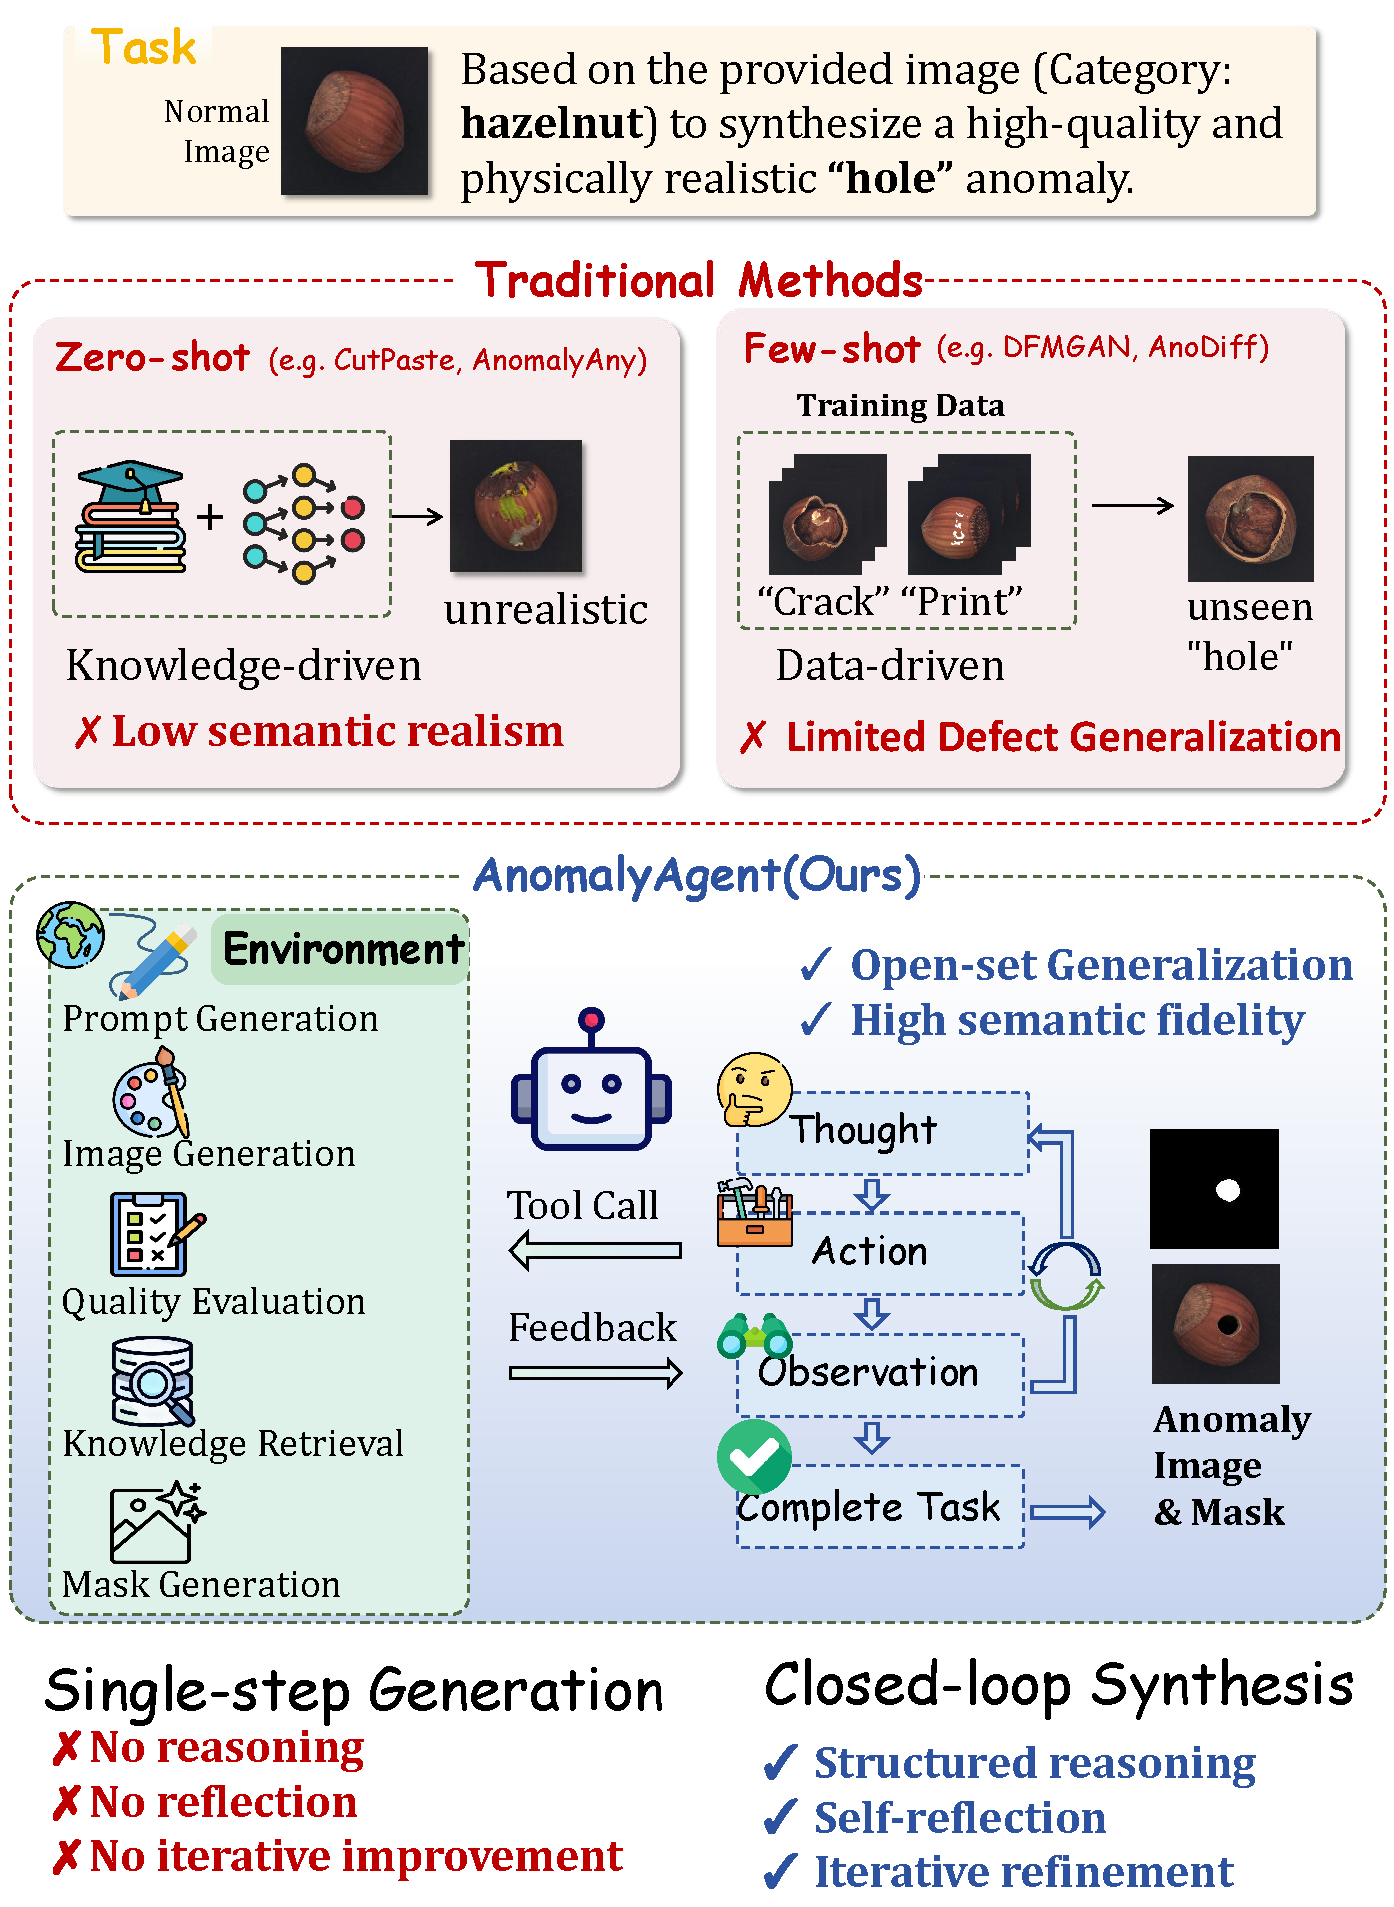
\includegraphics[height=29.6cm]{motivation.pdf}\par
\vspace{0.7cm}
\raggedright
% Paper: Introduction, paragraphs 1--4.
\lead{The challenge.} Real defects are scarce and highly diverse.\par
\lead{Few-shot:} limited defect coverage.\\
\lead{Zero-shot:} often lack semantic realism.\par
\lead{Our idea.} Use feedback to guide iterative synthesis and self-refinement.
\end{block}
\end{column}
\separatorcolumn
\begin{column}{0.7045\paperwidth}
\begin{block}{2. Method}
\centering
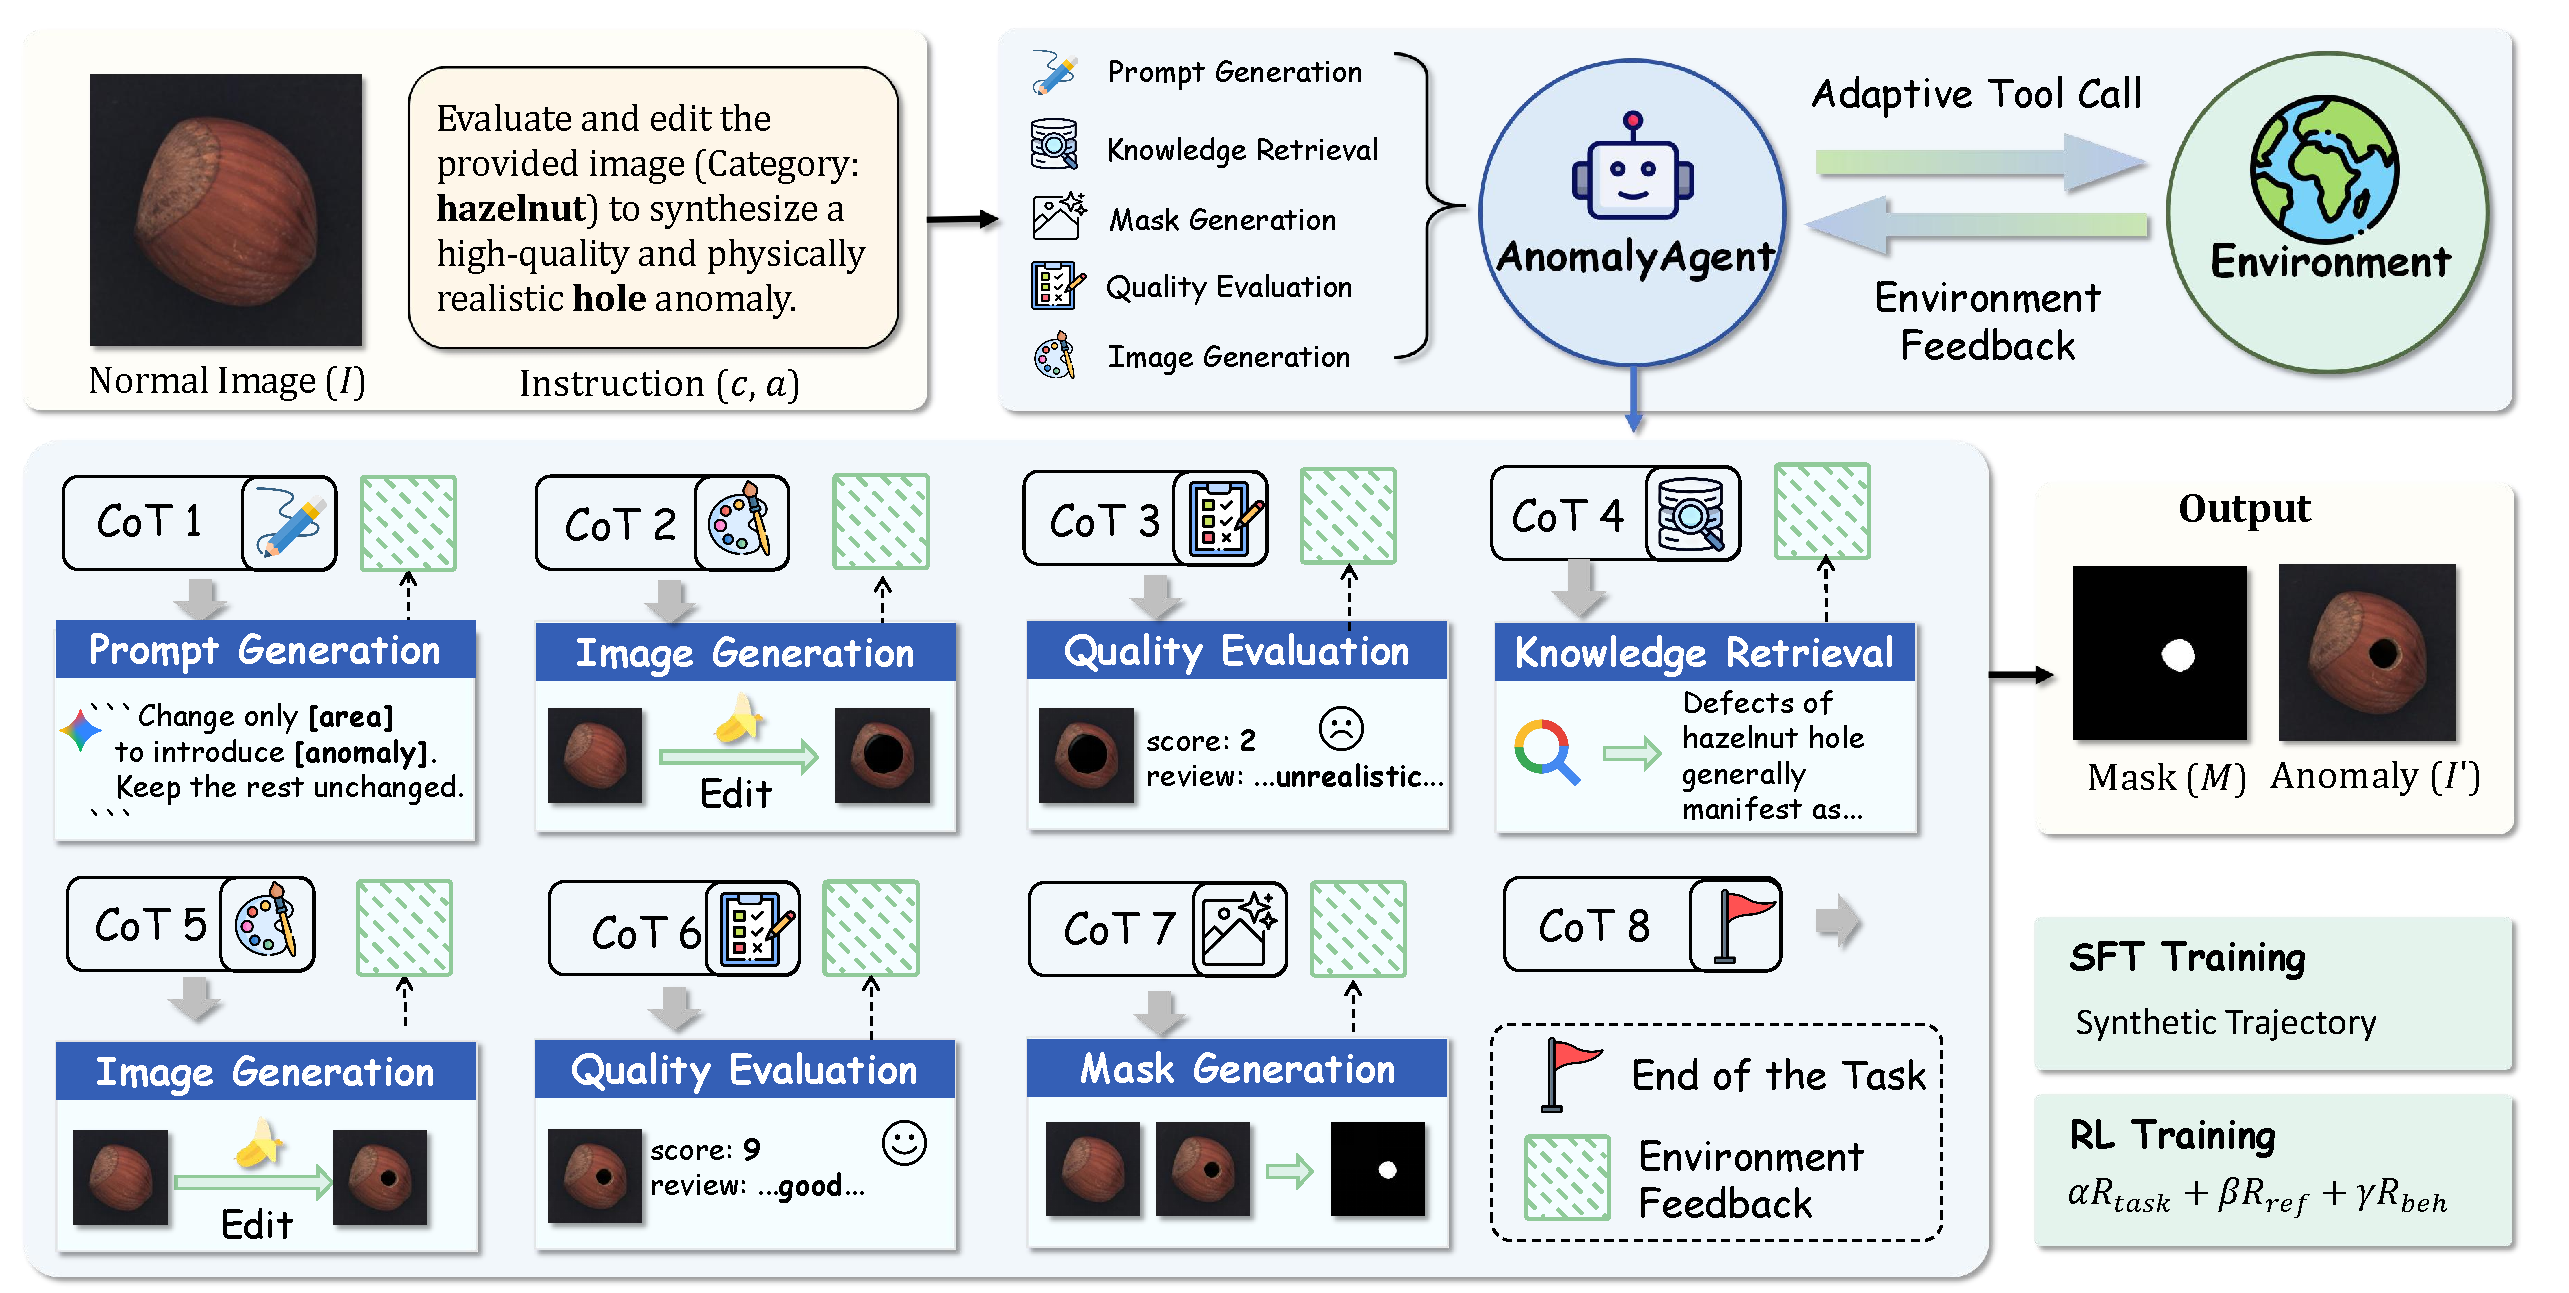
\includegraphics[height=29.6cm]{overview.pdf}\par
\vspace{0.7cm}
\raggedright
% Paper: Overview of AnomalyAgent; SFT; Agentic RL / Reward Design.
\lead{Adaptive tool use.} Given a normal image, its object category, and a target defect,
the agent dynamically selects among five tools to generate an anomaly image and its pixel-level mask.\par
\lead{Closed-loop refinement.} Quality scores and semantic feedback guide prompt
revision, with knowledge retrieval when needed. Tool selection adapts to the current state, not a fixed sequence.\par
\lead{Two-stage training.} SFT learns structured tool use from synthetic trajectories.
GRPO then optimizes long-horizon decision-making with \textbf{task, reflection, and behavior rewards.}
\end{block}
\end{column}
\separatorcolumn
\end{columns}
\vspace{0.4cm}
\begin{columns}[t]
\separatorcolumn
\begin{column}{\widewidth}
\begin{block}{3. Results}
% Measure both originals and use one shared height without stretching either.
\newcommand{\FullLocalizationTable}{%
\begingroup
\fontencoding{T1}\fontfamily{LinuxLibertineT-TLF}\fontseries{m}\fontsize{9}{10.8}\selectfont
\renewcommand{\arraystretch}{1}
\setlength{\tabcolsep}{1.5pt}

\begin{tabular}{l | ccc | ccc | ccc | ccc || ccc | ccc | ccc | ccc}
\toprule
\multirow{3}{*}{\textbf{Category}}
& \multicolumn{3}{c|}{AnoHybrid}
& \multicolumn{3}{c|}{Gemini-img}
& \multicolumn{3}{c|}{GPT-img}
& \multicolumn{3}{c||}{\textbf{AnomalyAgent}}
& \multicolumn{3}{c|}{AnoHybrid}
& \multicolumn{3}{c|}{Gemini-img}
& \multicolumn{3}{c|}{GPT-img}
& \multicolumn{3}{c}{\textbf{AnomalyAgent}} \\
\cmidrule(lr){2-4}\cmidrule(lr){5-7}\cmidrule(lr){8-10}\cmidrule(lr){11-13}
\cmidrule(lr){14-16}\cmidrule(lr){17-19}\cmidrule(lr){20-22}\cmidrule(lr){23-25}
& \multicolumn{12}{c||}{\textbf{Pixel-Level Performance}}
& \multicolumn{12}{c}{\textbf{Image-Level Performance}} \\
\cmidrule(lr){2-13}\cmidrule(lr){14-25}
& AUC & AP & \textit{F}\textsubscript{1} & AUC & AP & \textit{F}\textsubscript{1} & AUC & AP & \textit{F}\textsubscript{1} & AUC & AP & \textit{F}\textsubscript{1}
& AUC & AP & \textit{F}\textsubscript{1} & AUC & AP & \textit{F}\textsubscript{1} & AUC & AP & \textit{F}\textsubscript{1} & AUC & AP & \textit{F}\textsubscript{1} \\
\midrule
bottle & 98.3 & \textbf{77.2} & \textbf{72.5} & 96.1 & 74.5 & 68.1 & 86.0 & 52.7 & 51.5 & \textbf{97.2} & 73.5 & 69.7 & 99.2 & \textbf{99.8} & \textbf{98.7} & 98.7 & 99.5 & 97.7 & \textbf{99.5} & \textbf{99.8} & 97.7 & 98.7 & 99.6 & 98.1 \\
cable & 94.1 & 76.0 & \textbf{73.4} & 93.3 & 68.5 & 60.2 & 90.2 & 55.5 & 50.4 & \textbf{97.4} & \textbf{76.5} & 69.2 & 96.1 & 97.7 & 91.9 & 98.8 & 98.9 & 94.7 & 98.3 & 98.8 & \textbf{97.4} & \textbf{99.1} & \textbf{99.3} & 96.1 \\
capsule & \textbf{98.4} & \textbf{51.7} & \textbf{54.6} & 96.0 & 44.0 & 47.3 & 88.3 & 33.2 & 34.5 & 96.6 & 46.0 & 49.7 & \textbf{94.9} & \textbf{98.8} & \textbf{95.2} & 90.8 & 96.7 & 92.0 & 90.2 & 91.3 & 88.7 & 91.7 & 97.6 & 91.8 \\
carpet & 98.6 & 82.8 & 75.6 & 98.8 & 79.0 & 72.3 & 91.3 & 69.0 & 60.4 & \textbf{99.4} & \textbf{85.1} & \textbf{76.4} & 96.3 & 98.9 & 94.0 & 97.9 & 99.2 & 96.0 & 95.6 & 96.1 & 95.9 & \textbf{99.4} & \textbf{99.8} & \textbf{98.4} \\
grid & \textbf{98.8} & \textbf{58.6} & \textbf{59.2} & 97.4 & 27.5 & 38.6 & 89.0 & 22.1 & 32.7 & 97.8 & 40.3 & 44.9 & \textbf{100} & \textbf{100} & \textbf{100} & 95.6 & 98.0 & 93.7 & 95.7 & 98.0 & 93.7 & \textbf{100} & \textbf{100} & \textbf{100} \\
hazelnut & \textbf{99.6} & \textbf{89.4} & \textbf{82.6} & 96.7 & 81.1 & 77.4 & 90.3 & 78.3 & 70.2 & 99.4 & 86.4 & 80.1 & 96.7 & 98.3 & 92.6 & 96.2 & 97.0 & 90.4 & 94.1 & 97.9 & \textbf{96.0} & \textbf{98.9} & \textbf{99.2} & 95.9 \\
leather & 99.6 & 72.7 & 67.1 & 99.4 & 72.8 & 68.3 & 93.9 & 69.4 & 65.6 & \textbf{99.7} & \textbf{80.3} & \textbf{73.9} & 98.4 & 99.5 & 97.4 & \textbf{100} & \textbf{100} & \textbf{100} & 96.9 & 98.0 & 95.1 & \textbf{100} & \textbf{100} & \textbf{100} \\
metal nut & 98.8 & 93.5 & 87.0 & 97.5 & 90.6 & 83.6 & 86.2 & 58.5 & 58.6 & \textbf{99.3} & \textbf{95.4} & \textbf{88.5} & \textbf{99.8} & \textbf{99.9} & \textbf{99.2} & 99.4 & 99.8 & 97.7 & 95.5 & 98.6 & 93.5 & \textbf{99.8} & \textbf{99.9} & 98.7 \\
pill & 99.3 & \textbf{94.9} & \textbf{88.4} & 99.1 & 82.7 & 72.7 & 88.0 & 65.1 & 60.3 & \textbf{99.5} & 84.0 & 80.4 & \textbf{99.1} & \textbf{99.8} & \textbf{98.9} & 92.3 & 98.0 & 93.0 & 92.5 & 96.0 & 91.9 & 97.4 & 98.8 & 96.6 \\
screw & 77.0 & 7.8 & 6.4 & 97.6 & 10.5 & 17.3 & 94.7 & 21.6 & 29.9 & \textbf{98.4} & \textbf{55.4} & \textbf{57.8} & 44.6 & 72.6 & 84.9 & 88.4 & 94.5 & 88.1 & 90.9 & 95.3 & 88.6 & \textbf{94.6} & \textbf{97.8} & \textbf{91.3} \\
tile & 99.3 & \textbf{94.6} & \textbf{87.4} & 97.3 & 92.6 & 80.5 & 94.3 & 59.0 & 59.9 & \textbf{99.3} & \textbf{94.6} & 85.7 & 99.5 & 99.8 & 99.0 & 99.3 & 99.6 & 97.4 & 98.8 & 99.5 & 95.0 & \textbf{100} & \textbf{100} & \textbf{100} \\
toothbrush & 98.7 & 65.2 & 67.8 & \textbf{99.5} & \textbf{73.7} & \textbf{75.4} & 94.8 & 31.1 & 42.6 & 99.3 & 72.3 & 70.3 & \textbf{100} & \textbf{100} & \textbf{100} & \textbf{100} & \textbf{100} & \textbf{100} & 98.3 & 99.1 & 95.2 & \textbf{100} & \textbf{100} & \textbf{100} \\
transistor & \textbf{98.1} & \textbf{80.8} & \textbf{74.2} & 90.6 & 62.1 & 59.9 & 88.2 & 60.3 & 54.7 & 90.5 & 63.7 & 62.1 & 92.9 & 90.4 & 86.3 & 94.5 & 92.6 & 90.9 & 95.9 & \textbf{97.9} & \textbf{93.4} & \textbf{98.3} & 97.1 & 92.9 \\
wood & 95.8 & 70.7 & 64.8 & 95.8 & 78.5 & 72.8 & 82.2 & 45.6 & 49.0 & \textbf{97.5} & \textbf{79.8} & \textbf{74.0} & 96.6 & 98.7 & 98.7 & 98.5 & 99.3 & 97.7 & 97.3 & 98.0 & 94.3 & \textbf{100} & \textbf{100} & \textbf{100} \\
zipper & \textbf{99.1} & \textbf{82.3} & \textbf{74.9} & 96.9 & 75.8 & 66.4 & 90.4 & 55.0 & 49.4 & 98.9 & 79.8 & 72.4 & \textbf{99.9} & \textbf{100} & 99.3 & 99.2 & 99.7 & 97.0 & 96.3 & 98.1 & 94.2 & \textbf{99.9} & \textbf{100} & \textbf{99.4} \\
\midrule
\textbf{Mean} & 96.9 & 72.9 & 69.1 & 96.8 & 67.6 & 64.1 & 89.9 & 51.8 & 51.3 & \textbf{98.0} & \textbf{74.2} & \textbf{70.3} & 94.3 & 96.9 & 95.7 & 96.6 & 98.2 & 95.1 & 95.7 & 97.5 & 94.0 & \textbf{98.5} & \textbf{99.3} & \textbf{97.3} \\
\bottomrule
\end{tabular}
\endgroup}

\newsavebox{\resulttablebox}
\newsavebox{\resultimagebox}
\sbox{\resulttablebox}{\FullLocalizationTable}
\sbox{\resultimagebox}{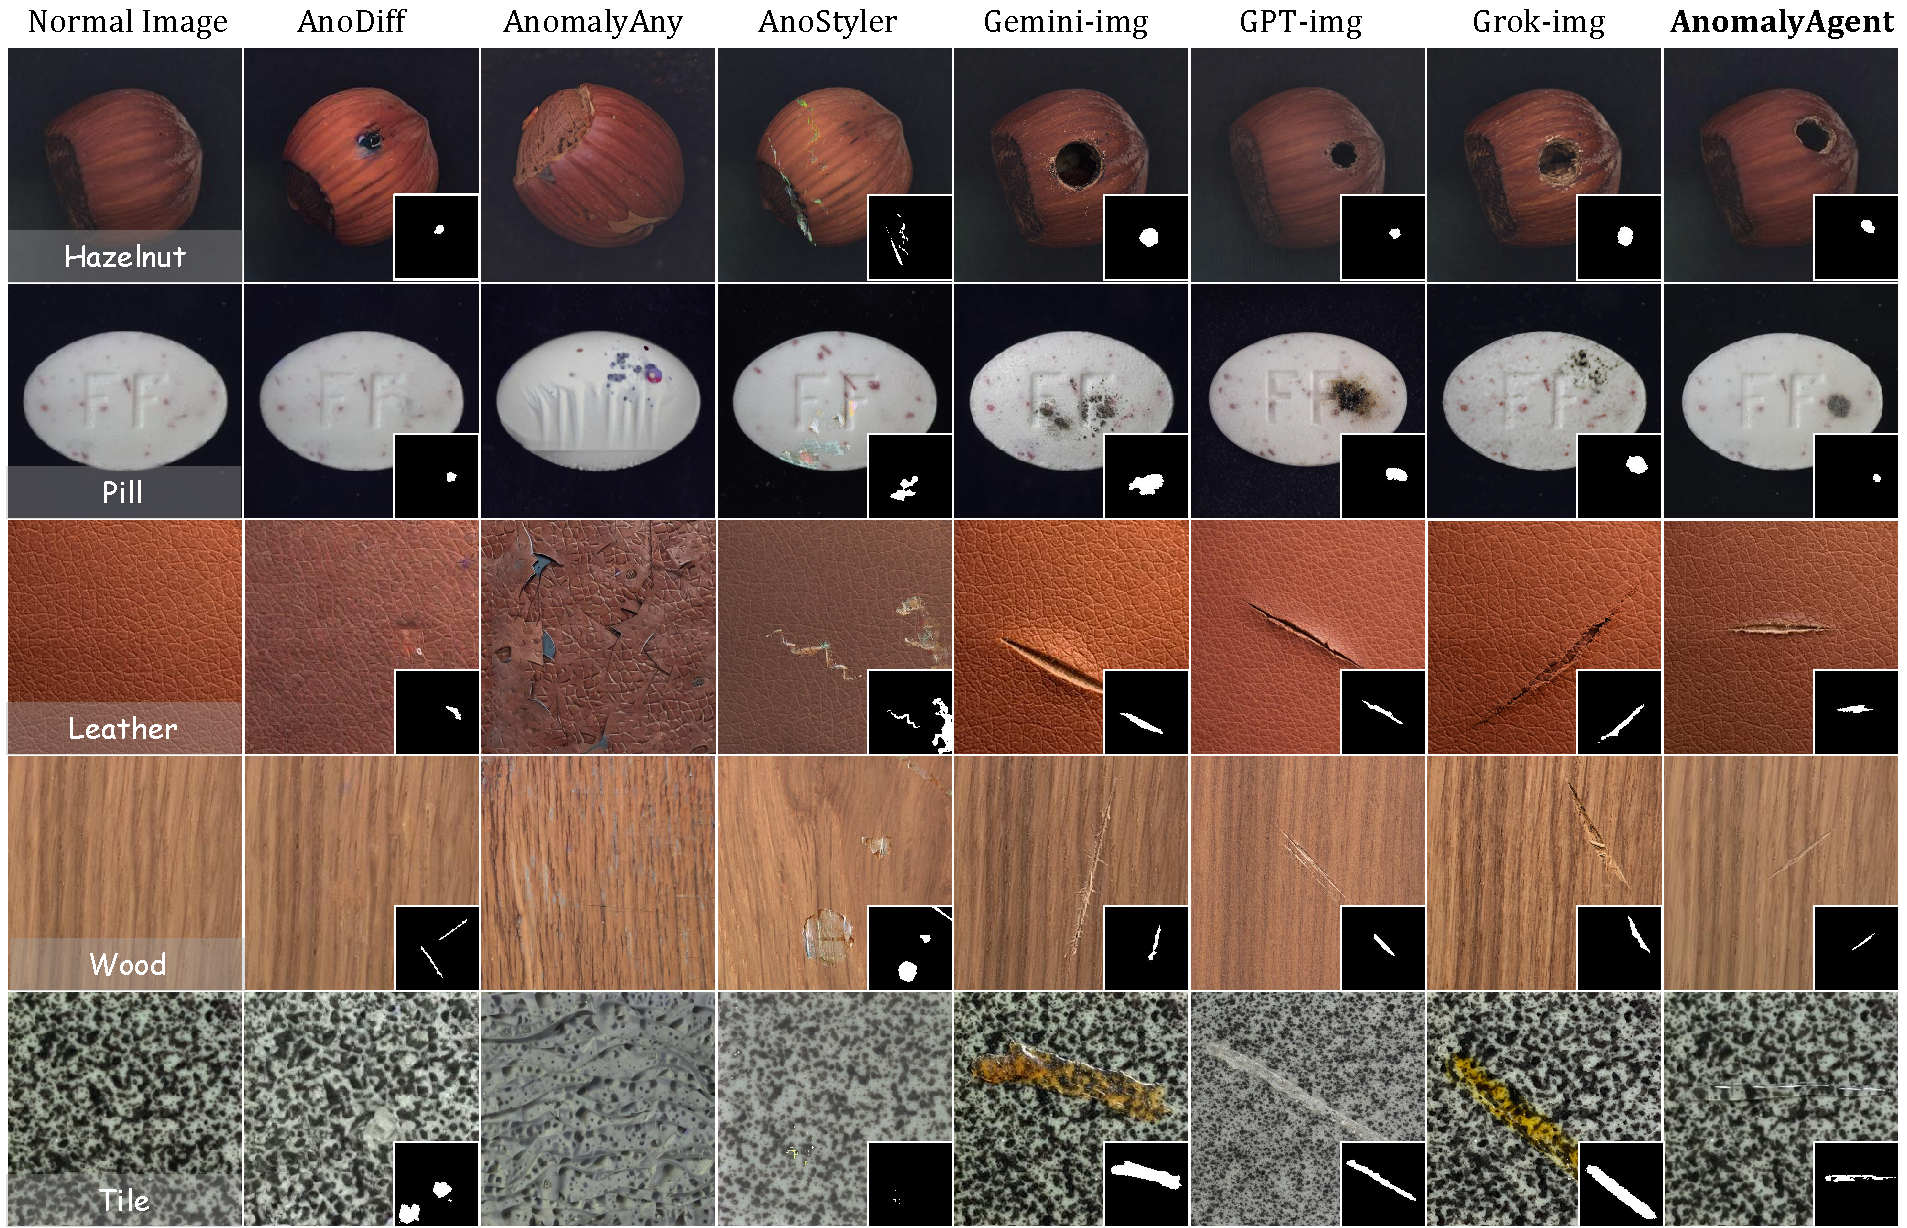
\includegraphics{vis_comparison.pdf}}
\pgfmathsetmacro{\resulttableratio}{\wd\resulttablebox/(\ht\resulttablebox+\dp\resulttablebox)}
\pgfmathsetmacro{\resultimageratio}{\wd\resultimagebox/(\ht\resultimagebox+\dp\resultimagebox)}
\pgfmathsetlengthmacro{\resultheight}{0.98*\linewidth/(\resulttableratio+\resultimageratio)}
\pgfmathsetlengthmacro{\resulttablewidth}{\resultheight*\resulttableratio}
\pgfmathsetlengthmacro{\resultimagewidth}{\resultheight*\resultimageratio}
\typeout{RESULTS: height=\resultheight, table width=\resulttablewidth, image width=\resultimagewidth}
\pgfmathsetmacro{\resultscale}{\resultheight/(\ht\resulttablebox+\dp\resulttablebox)}

% Tighten this section only; preserve the aligned table/image dimensions.
\vspace{-1.1cm}
\noindent
\begin{minipage}[t]{\resulttablewidth}
\vspace{0pt}
\resizebox*{!}{\resultheight}{\usebox{\resulttablebox}}\par
\vspace{0.8cm}
\raggedright
% Paper: Main Results / Anomaly Detection Results and Table localization.
\lead{Localization on MVTec-AD.} Best mean performance across all six metrics.\par
\textbf{98.0 pixel AUC / 98.5 image AUC.}
Pixel AP rises from 72.9 to \textbf{74.2} over AnoHybrid, providing more accurate spatial supervision for downstream detection.
\end{minipage}\hfill
\begin{minipage}[t]{\resultimagewidth}
\vspace{0pt}
\centering
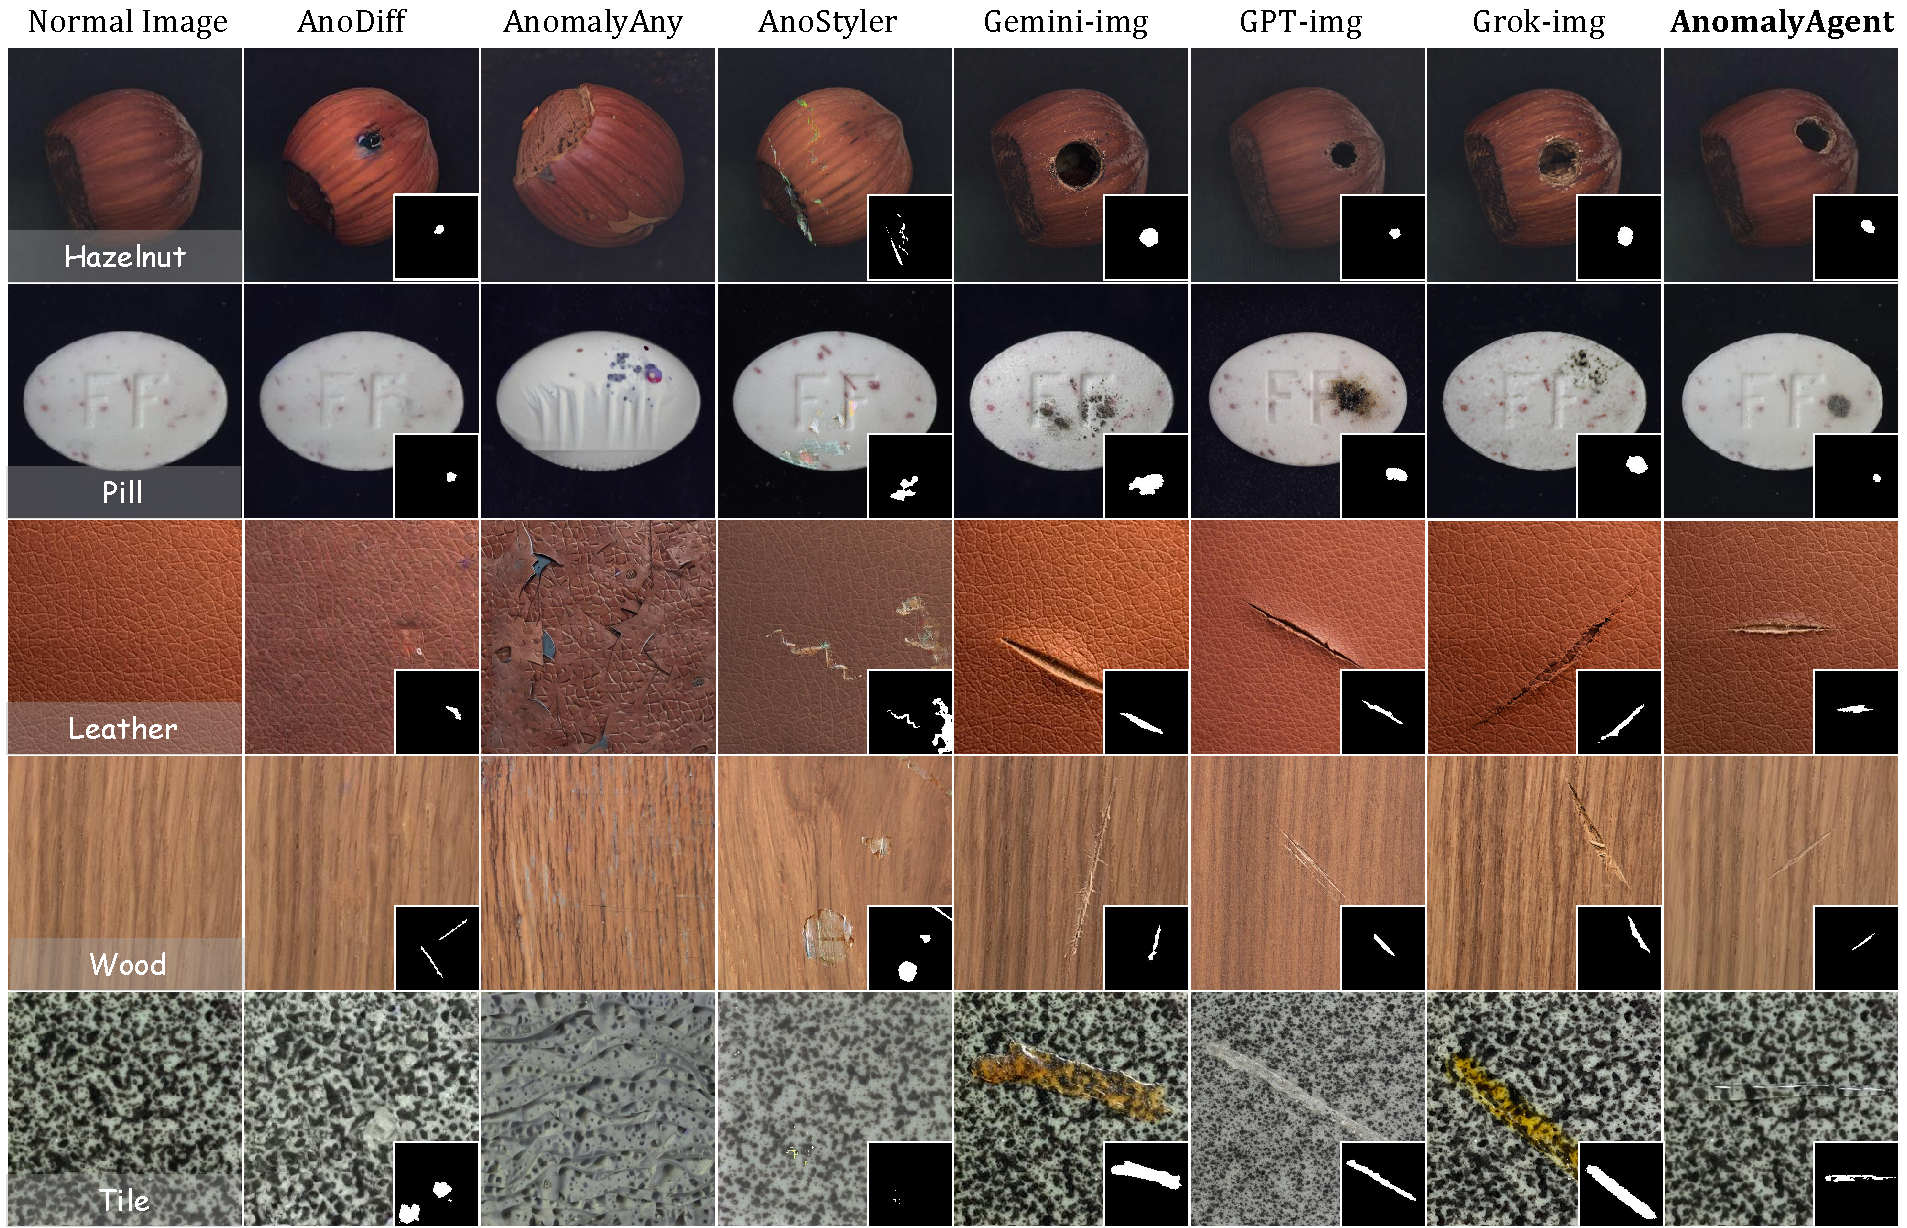
\includegraphics[height=\resultheight]{vis_comparison.pdf}\par
\vspace{0.8cm}
\raggedright
% Paper: Visualization Results.
\lead{Realistic defects. Precise masks.}\par
Iterative tool-driven refinement reduces semantic drift and incoherent defect boundaries.\par
\end{minipage}
\par\vspace{0.7cm}
% Same text size as localization; adjust row spacing, never font size,
% to align the two tables and the training curves at both edges.
% Paper result tables; scale both by exactly the localization scale.
\newcommand{\PosterGeneration}{%
\begingroup
\fontencoding{T1}\fontfamily{LinuxLibertineT-TLF}\fontseries{m}\fontsize{9}{10.8}\selectfont
\setlength{\tabcolsep}{8pt}
\renewcommand{\arraystretch}{1}
\begin{tabular}{l|c|c}
\toprule
\textbf{Method} & \textbf{IS$\uparrow$} & \textbf{IC-L$\uparrow$} \\
\midrule
CutPaste & 1.76 & 0.22 \\
DRAEM & 1.76 & 0.25 \\
NSA & 1.44 & 0.26 \\
RealNet & 1.64 & 0.22 \\
AnomalyAny & 2.02 & \textbf{0.33} \\
AnoStyler & 2.04 & \underline{0.32} \\
AnoHybrid & \underline{2.06} & \underline{0.32} \\
\midrule
Gemini-img & 1.91 & 0.29 \\
GPT-img & 1.77 & 0.29 \\
Grok-img & 1.68 & 0.28 \\
\midrule
\rowcolor{cyan!5}
\textbf{AnomalyAgent} & \textbf{2.10} & \textbf{0.33} \\
\bottomrule
\end{tabular}
\endgroup}
\newcommand{\PosterClassification}{%
\begingroup
\fontencoding{T1}\fontfamily{LinuxLibertineT-TLF}\fontseries{m}\fontsize{9}{10.8}\selectfont
\setlength{\tabcolsep}{2pt}
\renewcommand{\arraystretch}{\classificationstretch}
\begin{tabular}{l|c}
\toprule
\textbf{Method} & \textbf{Accuracy $\uparrow$} \\
\midrule
AnoStyler & 32.2 \\
AnoHybrid      & \underline{52.6} \\
\midrule
Gemini-img & 44.7 \\
GPT-img & 40.5 \\
Grok-img & 38.9 \\
\midrule
\rowcolor{cyan!5} 
\textbf{AnomalyAgent}                & \textbf{57.0} \\
\bottomrule
\end{tabular}
\endgroup}

\newsavebox{\generationbox}
\newsavebox{\classificationbox}
\def\classificationstretch{1}
\sbox{\generationbox}{\PosterGeneration}
\sbox{\classificationbox}{\PosterClassification}
\pgfmathsetmacro{\classificationstretch}{1+((\ht\generationbox+\dp\generationbox)-(\ht\classificationbox+\dp\classificationbox))/(7*10.8)}
\sbox{\classificationbox}{\PosterClassification}
\pgfmathsetlengthmacro{\extrarowheight}{\resultscale*(\ht\generationbox+\dp\generationbox)}
\typeout{EXTRA RESULTS: scale=\resultscale, height=\extrarowheight}
\newsavebox{\trainingbox}
\sbox{\trainingbox}{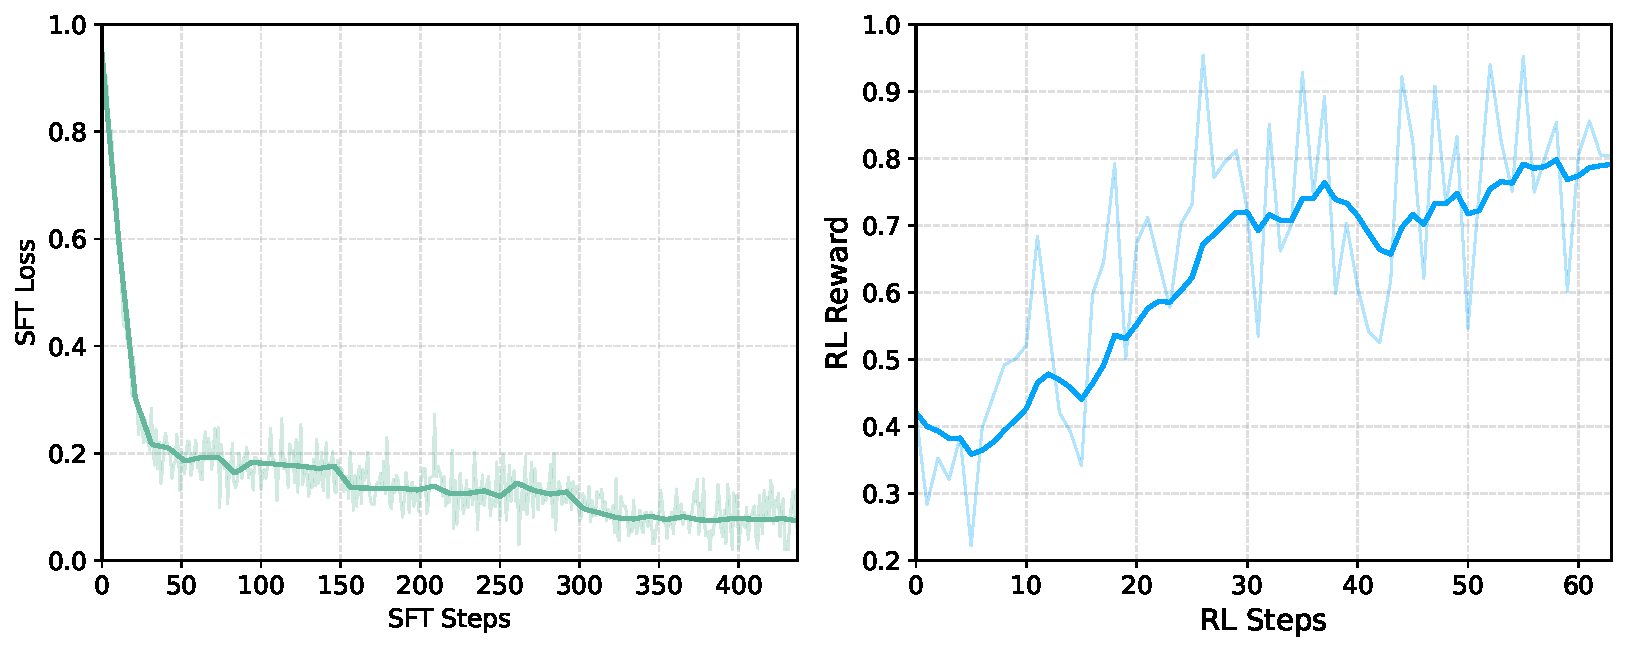
\includegraphics[height=\extrarowheight]{training_results.pdf}}
\pgfmathsetlengthmacro{\resultnotewidth}{\linewidth-\resultscale*(\wd\generationbox+\wd\classificationbox)-\wd\trainingbox-2.5cm}
\noindent\hbox to \linewidth{\scalebox{\resultscale}{\usebox{\generationbox}}\hspace{0.8cm}%
\scalebox{\resultscale}{\usebox{\classificationbox}}\hspace{0.8cm}%
\raisebox{-\resultscale\dp\generationbox}{\usebox{\trainingbox}}\hspace{0.8cm}%
\raisebox{-\resultscale\dp\generationbox}{%
\begin{minipage}[b][\extrarowheight][t]{\resultnotewidth}
% Paper: Main Results and Training Dynamics. All gains are percentage points.
\raggedright\fontsize{34}{42}\selectfont
\lead{Generation quality}\par
\textbf{2.10 IS}; joint-best \textbf{0.33 IC-L}.\par
\vspace{0.35cm}
\lead{Classification}\par
\textbf{57.0\%} accuracy; \textbf{+4.4 points} over AnoHybrid.\par
\vspace{0.35cm}
\lead{Training dynamics}\par
SFT loss converges; GRPO reward rises from \textbf{0.42 to 0.79}.
\end{minipage}}\hfil}\par
\end{block}
\end{column}
\separatorcolumn
\end{columns}
\vspace{0.3cm}
\begin{columns}[t]
\separatorcolumn
\begin{column}{\widewidth}
\begin{block}{4. Conclusion}
% The final block needs less trailing padding than inter-section blocks.
\setbeamertemplate{block end}{\end{beamercolorbox}\vspace{0.3cm}}
% Paper: Conclusion (including the stated future direction).
{\centering\fontsize{40}{49}\selectfont\lead{Anomaly synthesis as multi-turn decision-making.}\par}
\justifying
\fontsize{36}{42}\selectfont
AnomalyAgent integrates \textbf{structured tool use and iterative reasoning} for controllable,
semantically consistent anomaly generation beyond single-step pipelines. \textbf{SFT on synthetic
trajectories} teaches tool-use strategies, while \textbf{agentic RL} optimizes long-horizon decisions.
Experiments demonstrate \textbf{improved generation quality} and \textbf{stronger downstream classification
and localization} over existing zero-shot methods. Future work will scale to more complex
industrial scenarios and broader multimodal generation tasks.
\end{block}
\end{column}
\separatorcolumn
\end{columns}
\end{frame}
\end{document}
